\documentclass[10pt, letterpaper]{article}

% Packages:
\usepackage[
    ignoreheadfoot, % set margins without considering header and footer
    top=2 cm, % seperation between body and page edge from the top
    bottom=2 cm, % seperation between body and page edge from the bottom
    left=2 cm, % seperation between body and page edge from the left
    right=2 cm, % seperation between body and page edge from the right
    footskip=1.0 cm, % seperation between body and footer
    % showframe % for debugging 
]{geometry} % for adjusting page geometry
\usepackage[explicit]{titlesec} % for customizing section titles
\usepackage{tabularx} % for making tables with fixed width columns
\usepackage{array} % tabularx requires this
\usepackage[dvipsnames]{xcolor} % for coloring text
\definecolor{primaryColor}{RGB}{0, 79, 144} % define primary color
\usepackage{enumitem} % for customizing lists
\usepackage{fontawesome5} % for using icons
\usepackage{amsmath} % for math
\usepackage{graphicx}  % 用於插入圖片
\usepackage{subfig} % 用於並排圖片
\usepackage{subcaption} %並排放置圖片
\usepackage{caption}   % 控制 caption 格式
\usepackage{xeCJK}  % 支持中文
\usepackage{lastpage}
%\setCJKmainfont{NotoSansCJKtc-Regular}  % 或其他中文字體
\usepackage[
    pdftitle={Hua Liu's CV},
    pdfauthor={Hua Liu},
    pdfcreator={LaTeX with CV},
    colorlinks=true,
    urlcolor=primaryColor
]{hyperref} % for links, metadata and bookmarks
\usepackage[pscoord]{eso-pic} % for floating text on the page
\usepackage{calc} % for calculating lengths
\usepackage{bookmark} % for bookmarks
\usepackage{lastpage} % for getting the total number of pages
\usepackage{changepage} % for one column entries (adjustwidth environment)
\usepackage{paracol} % for two and three column entries
\usepackage{ifthen} % for conditional statements
\usepackage{needspace} % for avoiding page brake right after the section title
\usepackage{iftex} % check if engine is pdflatex, xetex or luatex

% Ensure that generate pdf is machine readable/ATS parsable:
\ifPDFTeX
    \input{glyphtounicode}
    \pdfgentounicode=1
    \usepackage[T1]{fontenc}
    \usepackage[utf8]{inputenc}
    \usepackage{lmodern}
\fi

\usepackage[default, type1]{sourcesanspro} 

% Some settings:
\AtBeginEnvironment{adjustwidth}{\partopsep0pt} % remove space before adjustwidth environment
\pagestyle{empty} % no header or footer
\setcounter{secnumdepth}{0} % no section numbering
\setlength{\parindent}{0pt} % no indentation
\setlength{\topskip}{0pt} % no top skip
\setlength{\columnsep}{0.15cm} % set column seperation
\makeatletter
\let\ps@customFooterStyle\ps@plain % Copy the plain style to customFooterStyle
\patchcmd{\ps@customFooterStyle}{\thepage}{
    \color{gray}\textit{\small Hua Liu - Page \thepage{} of \pageref*{LastPage}}
}{}{} % replace number by desired string
\makeatother
\pagestyle{customFooterStyle}

\titleformat{\section}{
    % avoid page braking right after the section title
    \needspace{4\baselineskip}
    % make the font size of the section title large and color it with the primary color
    \Large\color{primaryColor}
}{
}{
}{
    % print bold title, give 0.15 cm space and draw a line of 0.8 pt thickness
    % from the end of the title to the end of the body
    \textbf{#1}\hspace{0.15cm}\titlerule[0.8pt]\hspace{-0.1cm}
}[] % section title formatting

\titlespacing{\section}{
    % left space:
    -1pt
}{
    % top space:
    0.3 cm
}{
    % bottom space:
    0.2 cm
} % section title spacing

% \renewcommand\labelitemi{$\vcenter{\hbox{\small$\bullet$}}$} % custom bullet points
\newenvironment{highlights}{
    \begin{itemize}[
        topsep=0.10 cm,
        parsep=0.10 cm,
        partopsep=0pt,
        itemsep=0pt,
        leftmargin=0.4 cm + 10pt
    ]
}{
    \end{itemize}
} % new environment for highlights

\newenvironment{highlightsforbulletentries}{
    \begin{itemize}[
        topsep=0.10 cm,
        parsep=0.10 cm,
        partopsep=0pt,
        itemsep=0pt,
        leftmargin=10pt
    ]
}{
    \end{itemize}
} % new environment for highlights for bullet entries


\newenvironment{onecolentry}{
    \begin{adjustwidth}{
        0.2 cm + 0.00001 cm
    }{
        0.2 cm + 0.00001 cm
    }
}{
    \end{adjustwidth}
} % new environment for one column entries

\newenvironment{twocolentry}[2][]{
    \onecolentry
    \def\secondColumn{#2}
    \setcolumnwidth{\fill, 4.5 cm}
    \begin{paracol}{2}
}{
    \switchcolumn \raggedleft \secondColumn
    \end{paracol}
    \endonecolentry
} % new environment for two column entries

\newenvironment{threecolentry}[3][]{
    \onecolentry
    \def\thirdColumn{#3}
    \setcolumnwidth{1 cm, \fill, 4.5 cm}
    \begin{paracol}{3}
    {\raggedright #2} \switchcolumn
}{
    \switchcolumn \raggedleft \thirdColumn
    \end{paracol}
    \endonecolentry
} % new environment for three column entries

\newenvironment{header}{
    \setlength{\topsep}{0pt}\par\kern\topsep\centering\color{primaryColor}\linespread{1.5}
}{
    \par\kern\topsep
} % new environment for the header

\newcommand{\placelastupdatedtext}{% \placetextbox{<horizontal pos>}{<vertical pos>}{<stuff>}
  \AddToShipoutPictureFG*{% Add <stuff> to current page foreground
    \put(
        \LenToUnit{\paperwidth-2 cm-0.2 cm+0.05cm},
        \LenToUnit{\paperheight-1.0 cm}
    ){\vtop{{\null}\makebox[0pt][c]{
        \small\color{gray}\textit{Last updated in December 2024}\hspace{\widthof{Last updated in November 2024}}
    }}}%
  }%
}%

% save the original href command in a new command:
\let\hrefWithoutArrow\href

% new command for external links:
\renewcommand{\href}[2]{\hrefWithoutArrow{#1}{\ifthenelse{\equal{#2}{}}{ }{#2 }\raisebox{.15ex}{\footnotesize \faExternalLink*}}}


%%%%%%%%%%%%%%%%%%%%%%%%%%%%%%%%%%%%%%%%%%%%%%%%%%%%%%%%%%%%%
%                                                           %
%                      文件開始                              %
%                                                           %
%%%%%%%%%%%%%%%%%%%%%%%%%%%%%%%%%%%%%%%%%%%%%%%%%%%%%%%%%%%%%

\begin{document}
   
    \newcommand{\AND}{\unskip
        \cleaders\copy\ANDbox\hskip\wd\ANDbox
        \ignorespaces
    }
    \newsavebox\ANDbox
    \sbox\ANDbox{}

    \placelastupdatedtext
    \begin{header}
        \fontsize{30 pt}{30 pt}
        \textbf{Hua(Flora) Liu}

        \vspace{0.3 cm}

        \normalsize
        \mbox{\hrefWithoutArrow{https://liu092111.github.io/eng}{{\footnotesize\faLink}\hspace*{0.13cm}Personal Homepage}}%
        \kern 0.25 cm%
        \AND%
        \kern 0.25 cm%
        \mbox{\hrefWithoutArrow{https://www.google.com/maps/place/Taoyuan,+Taiwan}{{\footnotesize\faMapMarker*}\hspace*{0.13cm}Taoyuan, Taiwan}}%
        \kern 0.25 cm%
        \AND%
        \kern 0.25 cm%
        \mbox{\hrefWithoutArrow{mailto:liu092111@gmail.com}{{\footnotesize\faEnvelope[regular]}\hspace*{0.13cm}liu092111@gmail.com}}%
        \kern 0.25 cm%
        \AND%
        \\\kern 0.25 cm%
        \mbox{\hrefWithoutArrow{https://liu092111.github.io/}{{\footnotesize\faLink}\hspace*{0.13cm}Chinese Homepage}}%
        \kern 0.25 cm%
        \AND%
        \kern 0.25 cm%
        \mbox{\hrefWithoutArrow{tel:(+886)908736900}{{\footnotesize\faPhone*}\hspace*{0.13cm}(+886)908736900}}%
        \kern 0.25 cm%
        \AND%
        \kern 0.25 cm%
        \mbox{\hrefWithoutArrow{https://www.linkedin.com/in/hua-liu-b8a905236/}{{\footnotesize\faLinkedinIn}\hspace*{0.13cm}Hua Liu}}%
        \kern 0.25 cm%
        \AND%
        \kern 0.25 cm%
        \mbox{\hrefWithoutArrow{https://github.com/liu092111}{{\footnotesize\faGithub}\hspace*{0.13cm}liu092111}}%
    \end{header}

    \vspace{0.3 cm - 0.3 cm}

%%%%%%%%%%%%%%%%%%%%%%%%%%%%%%%%%%%%%%%%%%%%%%%%%%
    \section{Quick Introduce}
       
        \begin{onecolentry}
            During my internships at the \href{https://www.deltaww.com/en-US/index}{Delta Electronics} Research Center and \href{https://www.sgs.com.tw/en/}{SGS} Taiwan Inspection Technology, I gained hands-on experience in \textbf{digital twin} development and \textbf{reliability testing}.  I successfully implemented the concept of \textbf{smart manufacturing}, and \textbf{industry 4.0} principles.  These experiences have strengthened my passion for industrial innovation, and I am eager to contribute my expertise to drive technological advancement in future projects. 
        \end{onecolentry}

        \vspace{0.2 cm}

%%%%%%%%%%%%%%%%%%%%%%%%%%%%%%%%%%%%%%%%%%%%%%%%%%%%%%
    \section{Skills}

        \begin{onecolentry}
            \textbf{Coding:} Python, Matlab, C++, LabVIEW, Simulink \end{onecolentry}

        \vspace{0.2 cm}

        \begin{onecolentry}
            \textbf{CAD:} Ansys, Solidworks, AutoCAD \end{onecolentry}

    
%%%%%%%%%%%%%%%%%%%%%%%%%%%%%%%%%%%%%%%%%%%%%%%%%%%%%%%%

    \section{Education}
       
        \begin{twocolentry}
        {\textbf{MS}\hspace{0.2cm}\includegraphics[height=0.9em]{fig/icon/NTU.png}}{
            %2024 – 2026
        }
            \textbf{National Taiwan University}, \\Engineering Science and Ocean Engineering (Electrical and Electronic Group)
            \begin{highlights}
                \item \textbf{Research Topic:}
                \item \textbf{Coursework:} DL, Control Systems, Electronics Experiments, Elasticity
            \end{highlights}
        \end{twocolentry}

        \begin{twocolentry}
        {\textbf{BS}\hspace{0.2cm}\includegraphics[height=0.9em]{fig/icon/NCKU.png}}{
            %2020 – 2024
        }
            \textbf{National Cheng Kung University}, Mechanical Engineering
            \begin{highlights}
                \item \textbf{Research Topic:} Development of SMC System for Vibration Control
                \item \textbf{Coursework:} Robot Design, Vibration Control, Numerical Analysis
            \end{highlights}
        \end{twocolentry}

%%%%%%%%%%%%%%%%%%%%%%%%%%%%%%%%%%%%%換頁%%%%%%%%%%%%%%%%%%%%%%%%%%%%%%%%%%%%%%%%%% 
    
    \section{Work Experience (1y)}        
        \begin{twocolentry}{
            \mbox{\hrefWithoutArrow{https://maps.app.goo.gl/RJEUNWf4F5W4aHwD6}{{\footnotesize\faMapMarker*}\hspace*{0.13cm}Taipei, Taiwan}}%

        Jul 2024 – Aug 2024
        }
            \includegraphics[height=1em]{fig/icon/Delta.jpg}\hspace{0.2cm}
            \textbf{Delta Electronics} \\
            \textbf{\href{https://brandnews.deltaww.com/en/BrandCircleDetail/2222f}{Lab for Digital Twin-Based of Optimization}, R\&D Engineer Intern}
            \begin{highlights}
                \item Developed Python scripts for Ansys automation
                \item Improved modeling flexibility and efficiency
                \item Created modular scripts for various geometric shapes
                \item Packaged scripts for easy user application 
            \end{highlights}
        \end{twocolentry}


        \vspace{0.2 cm}

        \begin{twocolentry}{
            \mbox{\hrefWithoutArrow{https://maps.app.goo.gl/u1YeE7bdKuAf1Mjj7}{{\footnotesize\faMapMarker*}\hspace*{0.13cm}Tainan, Taiwan}}%

        Sept 2023 – Apr 2024
        }
            \includegraphics[width=1.2em]{fig/icon/SGS.png}\hspace{0.2cm}
            \textbf{SGS Taiwan Inspection Technology} \\
            \textbf{\href{https://www.sgs.com.tw/en/service/page/4/2/42-reliability-laboratory-reliability-services/96-reliability-testing}{Reliability Laboratory}  , Semester Intern}
            \begin{highlights}
                \item Reliability tests (vibration, shock, HALT)
                \item Performed Ansys FEA on customer's product 
                \item Analyzed test data and compared with simulation
                \item Liaised with Ansys and NI vendors
            \end{highlights}
        \end{twocolentry}

        \vspace{0.2 cm}

        \begin{twocolentry}{
            \mbox{\hrefWithoutArrow{https://maps.app.goo.gl/UMr3Yb4jVptAPkeVA}{{\footnotesize\faMapMarker*}\hspace*{0.13cm}Taoyuan, Taiwan}}%

        Jul 2022 – Aug 2022 \\Jul 2020 - Aug 2020
        }
            \includegraphics[height=1em]{fig/icon/isha.jpg}\hspace{0.2cm}
            \textbf{Industrial Safety and Health Association of the R.O.C}  \\\textbf{Summer Intern}
            \begin{highlights}
                \item Assisted with industry analysis and report writing
                \item Supported safety course participants 
            \end{highlights}
        \end{twocolentry}


%%%%%%%%%%%%%%%%%%%%%%%%%%%%%%%%%%%%%換頁%%%%%%%%%%%%%%%%%%%%%%%%%%%%%%%%%%%%%%%%%% 
    
\vspace{0.3 cm - 0.3 cm}    
    
\section{Research}

    \begin{twocolentry}{
        
        \href{https://liu092111.github.io/eng/project/university_project.html}{web link}
    }
        \textbf{Research Topic (2023) \\Development of Control Systems for Vibration Control}
        \begin{highlights}
            \item Applied in Precision Machinery Field
            \item Objective: Suppress Vibration under High-Speed Motion
            \item Control Methods: Sliding Mode Control (SMC), PID Control
            \item Tools Used: Matlab, Simulink
        \end{highlights}
    \end{twocolentry}


    \vspace{0.2 cm}

\section{Projects}
    \begin{twocolentry}{}
        \textbf{Deep Learning (2024)}
            \begin{highlights}
                \item Physics-Informed Neural Network (PINN)
                \item Neural Style Transfer
                \item Convolution Neural Network (CNN)
                \item Hagen-Poiseuille flow regression
            \end{highlights}
    \end{twocolentry}
    
    \begin{twocolentry}{         \href{https://liu092111.github.io/eng/project/robot_design.html}{web link}
    }
        \textbf{Mechanical Project (2023) \\Gripper Robot and Transport Robot}
        \begin{highlights}
            \item Design a foot-shaped gripper robot and an EV3 transport robot
            \item Responsible for gripper design and laser cutting
            \item Silver medal in the annual grade poster competition.
        \end{highlights}
        \vspace{0.2 cm}
        \textbf{Automatic Control (2022) \\Robot Line Following and Maze Navigation}
        \begin{highlights}
            \item Using EV3 to control robot movement and avoid obstacles 
        \end{highlights} 
    \end{twocolentry}


    \vspace{0.2 cm}

    \begin{twocolentry}{
        \href{https://liu092111.github.io/eng/project/mechanical_design.html}{web link}
    }
        \textbf{Kinematics (2021) \\Motion of Gear Systems}
        \begin{highlights}
            \item Design the number of teeth and the module to avoid interference
            \item Tools used: Solidworks
        \end{highlights}
        \vspace{0.2 cm}
        \textbf{Mechanical Design (2022) \\Stress Analysis}
        \begin{highlights}
            \item Use software for analysis and compare with theoretical calculations.
            \item First place in class competition
            \item Tools used: Ansys, Solidworks
        \end{highlights}
        \vspace{0.2 cm}
        \textbf{Mechanical Drawing (2021)}
        \begin{highlights}
            \item Created engineering drawingusing SolidWorks
            \item Tools used: Solidworks
        \end{highlights}
    \end{twocolentry}

\section{Fundamental Knowledge}
    \begin{twocolentry}{
        \href{https://liu092111.github.io/eng/project/numerical_analysis.html}{web link}
    }
        \textbf{Numerical Analysis (2023)}
        \begin{highlights}
            \item Analyze curve fitting, regression, matrices, ODEs, PDEs
            \item Solve file/image processing, animation, simulation problems
        \end{highlights}
        \vspace{0.2 cm}
        \textbf{Instrumentation and Measurement (2023)}
        \begin{highlights}
            \item Monitor 5-axis machine signals at various speeds
            \item Design experiments, data acquisition, processing, analysis
            \item Tools used: LabVIEW, DAQ, Matlab
        \end{highlights} 
    \end{twocolentry}
%%%%%%%%%%%%%%%%%%%%%%%%%%%%%%%%%%%%%換頁%%%%%%%%%%%%%%%%%%%%%%%%%%%%%%%%%%%%%%%%%%        
    \newpage
    {\fontsize{30pt}{30pt} \textbf{Internship-- Delta Electronics}} % 標題
    
    \vspace{0.3cm}
    
    \section{R\&D Engineer Intern, Lab for Digital Twin-Based Optimization (2024)}
    \normalsize
    
    \begin{figure}[htbp]
        \begin{minipage}[c]{0.5\linewidth}
            \centering
            \includegraphics[width=0.8\textwidth]{fig/Delta Electronics/Delta Flow Chart.png.jpg}
            \caption{Flow Chart}
        \end{minipage}%
        \begin{minipage}[c]{0.5\linewidth}
            \centering
            \includegraphics[width=0.8\textwidth]{fig/Delta Electronics/generate coil.jpg}
            \caption{Generate Coil}
        \end{minipage}
%%----------------------------------圖片換行---------------------------------------%%

        \vspace{2.0cm}

        \begin{minipage}[t]{0.33\linewidth}
            \centering
            \includegraphics[width=1.0\textwidth]{fig/Delta Electronics/FEA analysis process.jpg}
            \caption{FEA Process}
        \end{minipage}
        \begin{minipage}[t]{0.33\linewidth}
            \centering
            \includegraphics[width=1.0\textwidth]{fig/Delta Electronics/quick call bottom.jpg}
            \caption{Tool Kit}
        \end{minipage}%
        \begin{minipage}[t]{0.33\linewidth}
            \centering
            \includegraphics[width=1.0\textwidth]{fig/Delta Electronics/input parameters.jpg}
            \caption{Input Parameters}
        \end{minipage}          
    \end{figure}
%%%%%%%%%%%%%%%%%%%%%%%%%%%%%%%%%%%%%換頁%%%%%%%%%%%%%%%%%%%%%%%%%%%%%%%%%%%%%%%%%%        

    \newpage
    {\fontsize{30pt}{30pt} \textbf{Internship-- SGS Technology}} % 標題
    
    \vspace{0.3cm}
    
    \section{Reliability Engineer Intern (2023)}

    \normalsize
    \mbox{\hrefWithoutArrow{https://github.com/liu092111/College_Portfolio/blob/0d5be6fa66553ebed94cd609794cb3832255d13b/SGS\%20Inspection\%20Intern/\%E5\%8F\%AF\%E9\%9D\%A0\%E5\%BA\%A6\%E6\%A9\%9F\%E5\%8F\%B0\%E7\%9B\%B8\%E9\%97\%9C\%E8\%B3\%87\%E6\%96\%99.pdf}{{\footnotesize\faLink}\hspace*{0.13 cm}Testing Information}}%
    \kern 0.25 cm%
    
    \begin{figure}[!b]
        \vspace{-1.8 cm} 
        \begin{minipage}[c]{0.33\linewidth}
            \centering
            \includegraphics[width=0.6\textwidth]{fig/SGS Intern/SGS流程圖.jpg}
            \caption{Flow Chart}
        \end{minipage}%
        \begin{minipage}[c]{0.33\linewidth}
            \centering
            \includegraphics[width=4.2cm]{fig/SGS Intern/Thermal Test.jpg} \\
            \includegraphics[width=4.2cm]{fig/SGS Intern/Vibration Test.jpg}
            \caption{\\Thermal \& Vibration Test}
        \end{minipage}%
        \begin{minipage}[c]{0.33\linewidth}
            \centering
            \includegraphics[width=4.2cm]{fig/SGS Intern/Shock Test.jpg} \\
                \includegraphics[width=3.2cm]{fig/SGS Intern/Salt Spray Test.jpg}
            \caption{\\Shock  \& Salt Spray Test}
        \end{minipage}
%%----------------------------------圖片換行---------------------------------------%%

        \vspace{0.1 cm}
        
        \begin{minipage}[c]{0.33\linewidth}
            \centering
            \includegraphics[width=0.8\textwidth]{fig/SGS Intern/Fan Drawing (Solidworks).png}
            \caption{Fan Drawing}
        \end{minipage} %
        \begin{minipage}[c]{0.33\linewidth}
            \centering
            \includegraphics[width=0.8\textwidth]{fig/SGS Intern/Structure.png}
            \caption{Structure Analysis}
        \end{minipage}%
        \begin{minipage}[c]{0.33\linewidth}
            \centering
            \includegraphics[width=0.8\textwidth]{fig/SGS Intern/Fan analylsis.png}
            \caption{Fan Analysis (Solidworks)}
        \end{minipage}
%%----------------------------------圖片換行---------------------------------------%%

        \vspace{0.1 cm}

        \begin{minipage}[t]{0.33\linewidth}
            \centering
            \includegraphics[width=0.8\textwidth]{fig/SGS Intern/Velictiy field.jpg} 
            \caption{Velocity Field}
        \end{minipage}%
        \begin{minipage}[t]{0.33\linewidth}
            \centering
            \includegraphics[width=0.8\textwidth]{fig/SGS Intern/Velocity field2.jpg}
            \caption{Velocity section}
        \end{minipage}%
        \begin{minipage}[t]{0.33\linewidth}
            \centering
            \includegraphics[width=0.7\textwidth]{fig/SGS Intern/Pressure.png}
            \caption{Pressure section}
        \end{minipage}
%%----------------------------------圖片換行---------------------------------------%%

        \vspace{0.1 cm}
        
        \begin{minipage}[c]{0.33\linewidth}
            \centering
            \includegraphics[width=0.8\textwidth]{fig/SGS Intern/Acoustic.png}
            \caption{Acoustic Analysis 1}
        \end{minipage}%
        \begin{minipage}[c]{0.33\linewidth}
            \centering
            \includegraphics[width=0.7\textwidth]{fig/SGS Intern/Acoustic2.png}
            \caption{Acoustic Analysis 2}
        \end{minipage}%
        \begin{minipage}[c]{0.33\linewidth}
            \centering
            \includegraphics[width=4cm]{fig/SGS Intern/labview.png} \\
            \includegraphics[width=4cm]{fig/SGS Intern/labview2.png}
            \caption{\\LabVIEW Interface}
        \end{minipage}
        \vspace{1.8cm} %底部距離
    \end{figure}
    
%%%%%%%%%%%%%%%%%%%%%%%%%%%%%%%%%%%%%換頁%%%%%%%%%%%%%%%%%%%%%%%%%%%%%%%%%%%%%%%%%%             
    
    \newpage
    {\fontsize{30pt}{30pt} \textbf{Monographic Study}} % 標題
    
    \vspace{0.3cm}
    
    \section{Vibration Control (2023)}

    \normalsize
    \mbox{\hrefWithoutArrow{https://github.com/liu092111/College_Portfolio/blob/21037b344b215ae4113d7bc832f132e269f00817/Monographic\%20study/Report/\%E5\%A4\%A7\%E5\%B0\%88\%E7\%94\%9F\%E8\%A8\%88\%E7\%95\%AB_\%E5\%8A\%89\%E6\%A8\%BA__\%E6\%9C\%9F\%E6\%9C\%AB\%E5\%A0\%B1\%E5\%91\%8A.pdf}{{\footnotesize\faLink}\hspace*{0.13cm}Research Project Final Report}}%
    \kern 0.25 cm%
    

    \begin{figure}[!b] % 保持在底部
        \vspace*{-1.5cm}  % 整體往上移動一點
        \begin{minipage}[c]{0.33\linewidth}
            \centering
            \includegraphics[width=0.7\textwidth]{fig/Monographic Study/專題流程圖.jpg}
            \caption{Flow Chart}
        \end{minipage}%
        \begin{minipage}[c]{0.33\linewidth}
            \centering
            \includegraphics[width=0.7\textwidth]{fig/Monographic Study/大專生海報.jpg}
            \caption{Final Poster}
        \end{minipage}%
        \begin{minipage}[c]{0.33\linewidth}
            \centering
            \includegraphics[width=4cm]{fig/Monographic Study/光學檢測平台示意圖.png} \\
            \includegraphics[width=4cm]{fig/Monographic Study/光學檢測平台示實際圖.png}
            \caption{\\Rubber Platform}
        \end{minipage}
%%----------------------------------圖片換行---------------------------------------%%

        \vspace{0.3cm}

        \begin{minipage}[c]{0.33\linewidth}
            \centering
            \includegraphics[width=0.7\textwidth]{fig/Monographic Study/光學檢測平台流程圖.png}
            \caption{Experimental Setup}
        \end{minipage}
        \begin{minipage}[c]{0.33\linewidth}
            \centering
            \includegraphics[width=1.0\textwidth]{fig/Monographic Study/研究方法.png}
            \caption{Experimental Method}
        \end{minipage}
        \begin{minipage}[c]{0.33\linewidth}
            \centering
            \includegraphics[width=3.8cm]{fig/Monographic Study/建立平台模型(主動平台).png} \\
            \includegraphics[width=3.8cm]{fig/Monographic Study/建立平台模型(橡膠軸承).png}
            \caption{\\Platform Model}
        \end{minipage}
%%----------------------------------圖片換行---------------------------------------%%

        \vspace{0.3cm}

        \begin{minipage}[c]{0.33\linewidth}
            \centering
            \includegraphics[width=4cm]{fig/Monographic Study/設計控制器.png} \\
            \includegraphics[width=4cm]{fig/Monographic Study/控制器模擬.png}
            \caption{\\Design \& Simulation}
        \end{minipage}
        \begin{minipage}[c]{0.33\linewidth}
            \centering
            \includegraphics[width=4.5cm]{fig/Monographic Study/控制實驗結果-1.jpg} 
            \caption{\\Experiment Result 1}
        \end{minipage}
        \begin{minipage}[c]{0.33\linewidth}
            \centering
            \includegraphics[width=4.5cm]{fig/Monographic Study/控制實驗結果-2.jpg} 
            \caption{\\Experiment Result 2}
        \end{minipage} 
        \vspace{1.5cm} % 加入底部邊距
    \end{figure}

%%%%%%%%%%%%%%%%%%%%%%%%%%%%%%%%%%%%%換頁%%%%%%%%%%%%%%%%%%%%%%%%%%%%%%%%%%%%%%%%%%        

    \newpage
    {\fontsize{30pt}{30pt} \textbf{Robot Design}} % 標題
    
    \vspace{0.3cm}
    
    \section{Robot Design Project (2022)}

    \normalsize
    \mbox{\hrefWithoutArrow{https://github.com/liu092111/College_Portfolio/blob/71e4be464adb2a4c50174f57073b5a7411a3f80e/Mechanical\%20Project/Robot\%20Design_Final\%20Report.pdf}{{\footnotesize\faLink}\hspace*{0.13cm}Detailed Documentation}}%
    \kern 0.25 cm%
    
    \begin{figure}[htbp]
        \begin{minipage}[c]{0.33\linewidth}
            \centering
            \includegraphics[width=0.8\textwidth]{fig/Robot Design/機專流程圖.jpg}
            \caption{Flow Chart}
        \end{minipage}%
        \begin{minipage}[c]{0.33\linewidth}
            \centering
            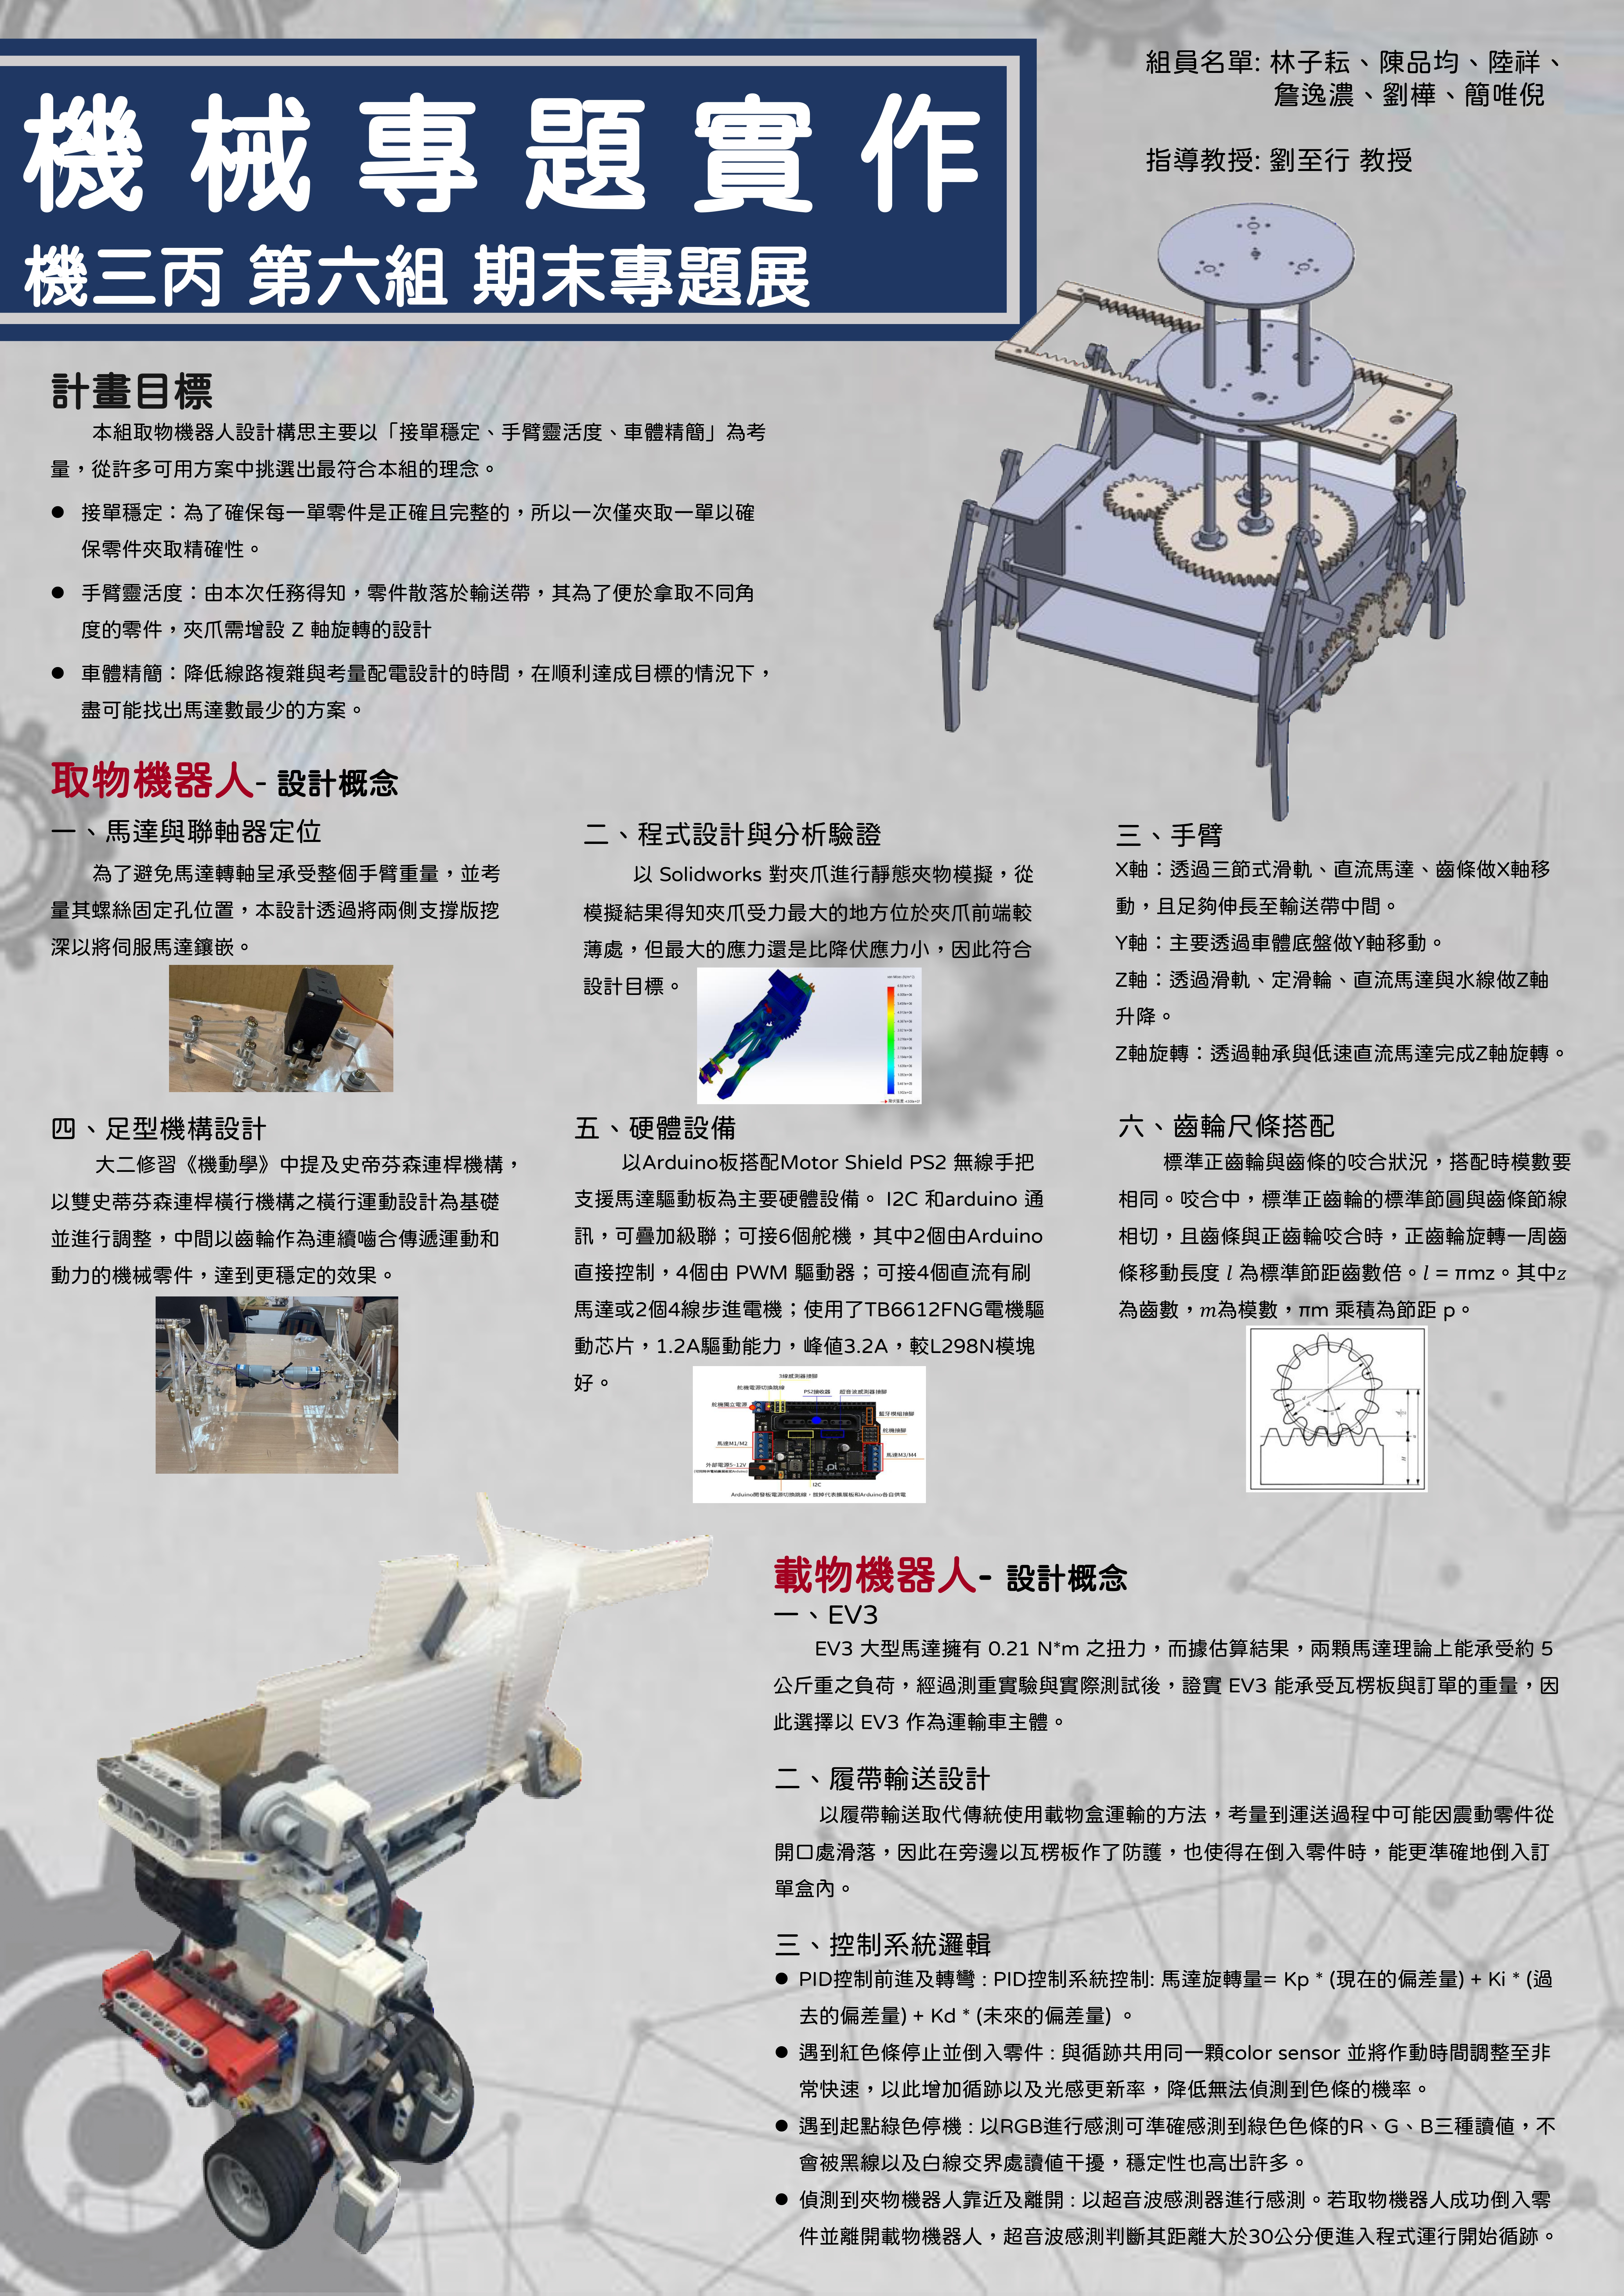
\includegraphics[width=0.8\textwidth]{fig/Robot Design/機械專題海報.jpg}
            \caption{Final Poster}
        \end{minipage}%
        \begin{minipage}[c]{0.33\linewidth}
            \centering
            \includegraphics[width=5cm]{fig/Robot Design/機器人設計.png}
            \caption{Robot Design}
        \end{minipage}         
%%----------------------------------圖片換行---------------------------------------%%

        \vspace{1.6cm}

        \begin{minipage}[c]{0.33\linewidth}
            \centering
            \includegraphics[width=0.8\textwidth]{fig/Robot Design/夾爪受力分析.png}
            \caption{Robot Analysis}
        \end{minipage}
        \begin{minipage}[c]{0.33\linewidth}
            \centering
            \includegraphics[width=0.8\textwidth]{fig/Robot Design/夾取物品.png}
            \caption{Gripping Component}
        \end{minipage}%
        \begin{minipage}[c]{0.33\linewidth}
            \centering
            \includegraphics[width=0.8\textwidth]{fig/Robot Design/物品交接.png}
            \caption{Transfer}
        \end{minipage}            
%%----------------------------------圖片換行---------------------------------------%%

        \vspace{1.6cm}

        \begin{minipage}[c]{0.33\linewidth}
            \centering
            \includegraphics[width=0.8\textwidth]{fig/Robot Design/運輸.png}
            \caption{Transport}
        \end{minipage}
        \begin{minipage}[c]{0.33\linewidth}
            \centering
            \includegraphics[width=0.8\textwidth]{fig/Robot Design/循跡.png}
            \caption{EV3 Line Following}
        \end{minipage}
        \begin{minipage}[c]{0.33\linewidth}
            \centering
            \includegraphics[width=0.8\textwidth]{fig/Robot Design/走迷宮.png}
            \caption{EV3 Navigating Maze}
        \end{minipage}            
    \end{figure}
%%%%%%%%%%%%%%%%%%%%%%%%%%%%%%%%%%%%%換頁%%%%%%%%%%%%%%%%%%%%%%%%%%%%%%%%%%%%%%%%%%             
        
    \newpage
    {\fontsize{30pt}{30pt} \textbf{Instrument \& Measurement}} % 標題

    \vspace{0.3cm}

    \section{Signal Process \& Numerical Analysis (2023)}

    \normalsize
    \mbox{\hrefWithoutArrow{https://github.com/liu092111/College_Portfolio/blob/0d5be6fa66553ebed94cd609794cb3832255d13b/Instrument\%20and\%20Measurement/Instrument\%20\%26\%20Measurement\%20Final\%20Report.pdf}{{\footnotesize\faLink}\hspace*{0.13cm} Instrument \& Measurement Final Report}}%
    \kern 0.25 cm%


    \begin{figure}[htbp] % 保持在底部
        \begin{minipage}[c]{0.33\linewidth}
            \centering
            \includegraphics[width=0.7\textwidth]{fig/Numerical Analysis/Numerical flow chart.jpg}
            \caption{Flow Chart}
        \end{minipage}%
        \begin{minipage}[c]{0.33\linewidth}
            \centering
            \includegraphics[width=0.7\textwidth]{fig/Numerical Analysis/五軸加工機.png}
            \caption{Five-Axis Processing Machine}
        \end{minipage}%
        \begin{minipage}[c]{0.33\linewidth}
            \centering
            \includegraphics[width=0.7\textwidth]{fig/Numerical Analysis/狀態監控流程圖.png}
            \caption{Condition Monitoring}
        \end{minipage}
    %%----------------------------------圖片換行---------------------------------------%%

        \vspace{0.9cm}

        \begin{minipage}[c]{0.33\linewidth}
            \centering
            \includegraphics[width=0.7\textwidth]{fig/Numerical Analysis/濾波前後時域訊號.png}
            \caption{Signal Process}
        \end{minipage}%
        \begin{minipage}[c]{0.33\linewidth}
            \centering
            \includegraphics[width=0.7\textwidth]{fig/Numerical Analysis/原始訊號和濾波訊號.png}
            \caption{Filtered Signal}
        \end{minipage}%
        \begin{minipage}[c]{0.33\linewidth}
            \centering
            \includegraphics[width=1.0\textwidth]{fig/Numerical Analysis/1000rpm, 5000rpm, 10000rpm 頻譜圖.png}
            \caption{Frequency Spectrum}
        \end{minipage}
    %%----------------------------------圖片換行---------------------------------------%%

        \vspace{0.9cm}

        \begin{minipage}[c]{0.33\linewidth}
            \centering
            \includegraphics[width=4.5cm]{fig/Numerical Analysis/以不同數值分析方法求解.png} 
            \caption{Numerical Analysis Methods}
        \end{minipage}%
        \begin{minipage}[c]{0.33\linewidth}
            \centering
            \includegraphics[width=4.5cm]{fig/Numerical Analysis/Rainfall station maps, Real-time Rainfall and Cumulative Rainfall.jpg} 
            \caption{Rainfall station map}
        \end{minipage}%
        \begin{minipage}[c]{0.33\linewidth}
            \centering
            \includegraphics[width=4.5cm]{fig/Numerical Analysis/隨機數製作高斯分布理論值.png} 
            \caption{Gaussian Distribution}
        \end{minipage} 
    \end{figure}

%%%%%%%%%%%%%%%%%%%%%%%%%%%%%%%%%%%%%換頁%%%%%%%%%%%%%%%%%%%%%%%%%%%%%%%%%%%%%%%%%%


    \newpage
    {\fontsize{30pt}{30pt} \textbf{Mechanical Design}} % 標題
    
    \vspace{0.3cm}
    
    \section{Kinematic Analysis (2022)}

    \normalsize
    \mbox{\hrefWithoutArrow{https://github.com/liu092111/College_Portfolio/blob/5ad988d0433266a348382bcdb4a4998478eef397/Mechanical\%20Design/\%E6\%A9\%9F\%E6\%A2\%B0\%E8\%A8\%AD\%E8\%A8\%88\%E6\%9C\%9F\%E6\%9C\%AB\%E6\%9B\%B8\%E9\%9D\%A2\%E5\%A0\%B1\%E5\%91\%8A.pdf}{{\footnotesize\faLink}\hspace*{0.13cm}Detailed Documentation}}%
    \kern 0.25 cm%
    
    \begin{figure}[!b]
        \vspace{-0.8 cm} 
        \begin{minipage}[c]{0.33\linewidth}
            \centering
            \includegraphics[width=0.6\textwidth]{fig/Mechanical Design/Mechanical Design Flow Chart.jpg}
            \caption{Flow Chart}
        \end{minipage}%
        \begin{minipage}[c]{0.33\linewidth}
            \centering
            \includegraphics[width=0.8\textwidth]{fig/Mechanical Design/齒輪系示意圖.png}
            \caption{Planet Gear System Diagram}
        \end{minipage}%
        \begin{minipage}[c]{0.33\linewidth}
            \centering
            \includegraphics[width=0.8\textwidth]{fig/Mechanical Design/齒輪系繪製.png}
            \caption{Gear System}
        \end{minipage} 
%%----------------------------------圖片換行---------------------------------------%%

        \vspace{0.5 cm}
        
        \begin{minipage}[c]{0.33\linewidth}
            \centering
            \includegraphics[width=0.8\textwidth]{fig/Mechanical Design/gear motion.jpg}
            \caption{Gear Motion}
        \end{minipage} %
        \begin{minipage}[c]{0.33\linewidth}
            \centering
            \includegraphics[width=0.8\textwidth]{fig/Mechanical Design/Solidworks應力位移分析.png}
            \caption{Stress Analysis}
        \end{minipage}%
        \begin{minipage}[c]{0.33\linewidth}
            \centering
            \includegraphics[width=0.8\textwidth]{fig/Mechanical Design/Ansys應力位移分析.png}
            \caption{Displacement Analysis}
        \end{minipage}
%%----------------------------------圖片換行---------------------------------------%%

        \vspace{0.5 cm}

        \begin{minipage}[c]{0.33\linewidth}
            \centering
            \includegraphics[width=4cm]{fig/Mechanical Design/簡化機構分析.png} 
            \caption{\\Simplify Structure}
        \end{minipage}%
        \begin{minipage}[c]{0.33\linewidth}
            \centering
            \includegraphics[width=0.8\textwidth]{fig/Mechanical Design/V8引擎.png}
            \caption{V8 Engine}
        \end{minipage}%
        \begin{minipage}[c]{0.33\linewidth}
            \centering
            \includegraphics[width=0.8\textwidth]{fig/Mechanical Design/拖車栓掛.png}
            \caption{Trailer Hitching}
        \end{minipage}%
%%----------------------------------圖片換行---------------------------------------%%

        \vspace{0.5 cm}
        
        \begin{minipage}[c]{0.33\linewidth}
            \centering
            \includegraphics[width=0.8\textwidth]{fig/Mechanical Design/萬象接頭.png}
            \caption{Universal Joint}
        \end{minipage}%
        \begin{minipage}[c]{0.33\linewidth}
            \centering
            \includegraphics[width=0.8\textwidth]{fig/Mechanical Design/萬象接頭之爆炸圖.png}
            \caption{Exploded View}
        \end{minipage}%
        \begin{minipage}[c]{0.33\linewidth}
            \centering
            \includegraphics[width=0.8\textwidth]{fig/Mechanical Design/游標卡尺.png}
            \caption{Vernier Caliper}
        \end{minipage}
        \vspace{0.8cm} %底部距離
    \end{figure}
%%%%%%%%%%%%%%%%%%%%%%%%%%%%%%%%%%%%%換頁%%%%%%%%%%%%%%%%%%%%%%%%%%%%%%%%%%%%%%%%%% 
   
\end{document}



    
    